\documentclass[12pt]{article}
\usepackage{graphicx}
\usepackage{amsmath}
\usepackage{geometry}
\usepackage{hyperref}
\geometry{margin=1in}

\title{Market Dynamics and Social Networks in Online Retail:\\
An Integrated Nash Equilibrium Analysis}
\author{Saeed Pakniat | 40139537\\
\small GitHub Repository: \url{https://github.com/AghoyPandaaa/OnlineMarketPlace_Simulation_GT_SN.git}}
\date{\today}

\begin{document}
\maketitle

\begin{abstract}
This report presents an integrated simulation study of price competition and social network effects in online retail. Using a real e-commerce transaction dataset, we model seller behavior, simulate Nash equilibrium with and without word-of-mouth effects, and quantify the added economic value of social influence. Our results demonstrate how network effects alter competitive dynamics and market outcomes.
\end{abstract}

\section{Introduction}
\begin{itemize}
    \item Briefly explain the motivation: understanding how prices, advertising, and word-of-mouth shape online retail markets.
    \item State goals: build realistic seller models, run game-theoretic simulations, quantify value of networks.
\end{itemize}

\section{Data and Preprocessing}
\begin{itemize}
    \item Source: UCI Online Retail Dataset.
    \item Preprocessing steps: data cleaning, merging, extracting relevant fields (Invoices, Prices, Quantities, Country, etc).
    \item Dataset summary: e.g., 407,664 rows, 9 columns. (Add table if wanted!)
\end{itemize}

\begin{figure}[h]
\centering
\includegraphics[width=0.85\textwidth]{../Task1/Task1_EDA_Results.png}
\caption{Exploratory Data Analysis: Distribution of key variables and outlier handling results.}
\end{figure}

\section{Seller Modeling}
\begin{itemize}
    \item Product selection criteria: chose top-selling products with price variation.
    \item Seller segmentation: Defined 3 price-tiered sellers (Low, Mid, High), each with empirically derived cost, price, demand, ad budget.
    \item Show statistics for each seller:
\end{itemize}

\begin{table}[h]
\centering
\begin{tabular}{lcccc}
\hline
Seller & Price Range & Avg Price & Base Demand & Total Revenue \\
\hline
Seller A & €1.90–€2.36 & €2.09 & 464   &  €2,000 \\
Seller B & €2.36–€2.95 & €2.55 & 53    &  €99,558 \\
Seller C & €2.95–€3.24 & €2.95 & 7     &  €50,066 \\
\hline
\end{tabular}
\caption{Key metrics for each seller segment.}
\end{table}

\begin{figure}[h]
\centering
\includegraphics[width=0.85\textwidth]{../Task2/seller_analysis.png}
\caption{Seller comparison: Average prices, total quantities, revenues, and price distributions.}
\end{figure}

\section{Market Model and Equilibrium Simulation}
\begin{itemize}
    \item Defined a MarketModel class; demand is affected by price, ads, and (in Network Mode) social influence.
    \item Parameters: 
        \begin{itemize}
            \item $\alpha$: advertising effectiveness ($0.01$)
            \item $\beta$: price sensitivity ($5.0$)
            \item $\epsilon$: price elasticity ($0.5$)
            \item $\gamma$: social influence (0 or 2.0)
        \end{itemize}
    \item Simulation process: iterative best-response for Nash equilibrium.
\end{itemize}

\section{Profit Landscape and Parameter Sensitivity}
\begin{itemize}
    \item Describe grid search for price and ad strategies, visualized as landscape (insert figure).
    \item Summarize how equilibrium profit moves for different $\alpha$ and $\beta$.
\end{itemize}
% Insert Figure Here (profit landscape, parameter sensitivity)
\begin{figure}[h]
\centering
\includegraphics[width=0.85\textwidth]{../Task3/profit_landscape.png}
\caption{Profit landscape for Seller A given competitor's fixed strategy.}
\end{figure}

\begin{figure}[h]
\centering
\includegraphics[width=0.85\textwidth]{../Task3/nash_equilibrium.png}
\caption{Nash equilibrium convergence: Price, ad budget, profit evolution and strategy trajectories.}
\end{figure}

\begin{figure}[h]
\centering
\includegraphics[width=0.75\textwidth]{../Task3/parameter_sensitivity.png}
\caption{Parameter sensitivity analysis showing impact of advertising effectiveness ($\alpha$) and price sensitivity ($\beta$) on profits.}
\end{figure}

\section{Social Network Analysis}
\begin{itemize}
    \item Constructed a customer influence network (e.g., PageRank, centrality, 500 nodes/64K edges).
    \item Quantified average influence per seller.
    \item Insert summary and network visualization if available.
\end{itemize}

\begin{figure}[h]
\centering
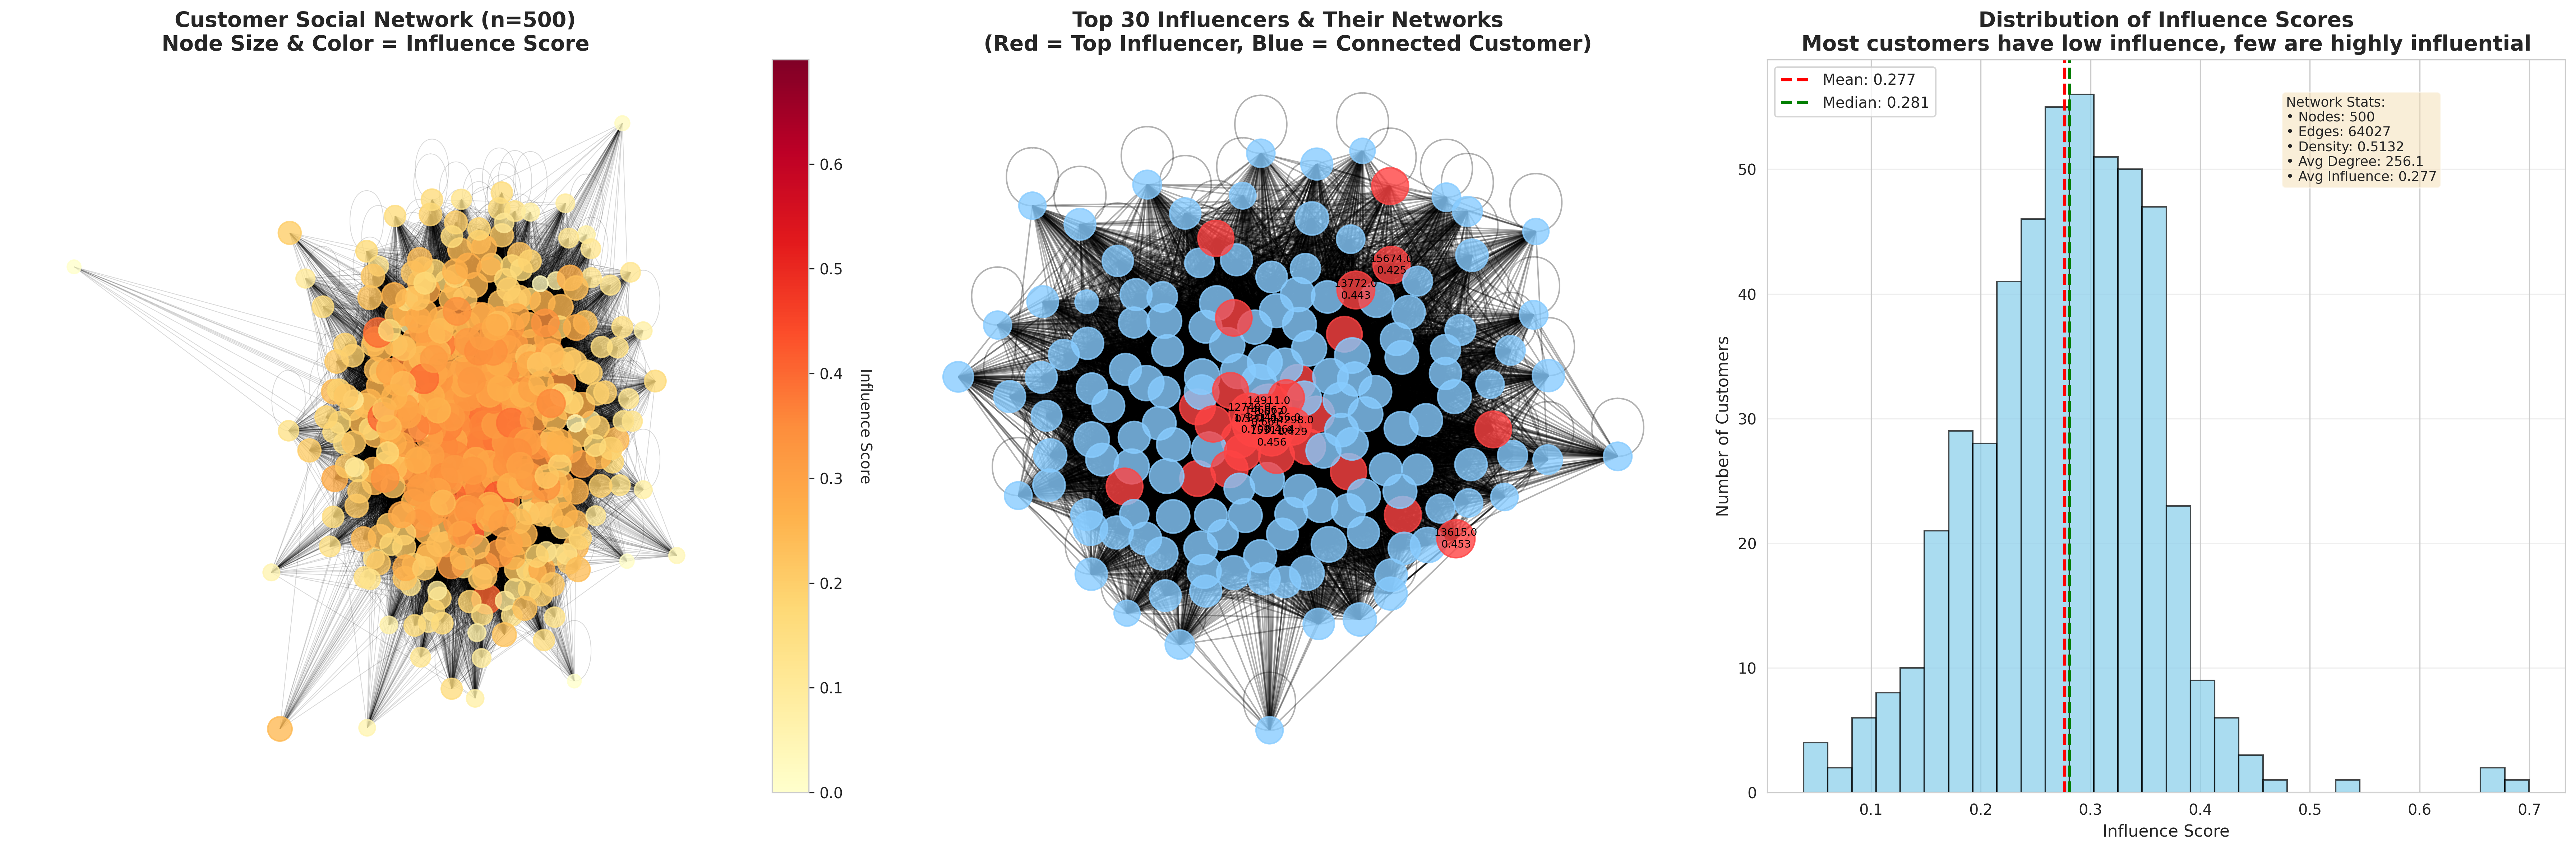
\includegraphics[width=0.75\textwidth]{../Task4/social_network.png}
\caption{Customer social network visualization showing influence connections and community structure.}
\end{figure}

\section{Integrated Simulation: Nash Equilibrium with Network Effects}
\begin{itemize}
    \item Compared equilibrium with $\gamma=0$ and with $\gamma=2.0$ (network influence).
    \item Main result: Social networks increased total profit by €1.83 (\textasciitilde0.6\%), skewed toward more influential sellers.
\end{itemize}
% Insert Final Comparison Figure Here
\begin{figure}[h]
\centering
\includegraphics[width=0.8\textwidth]{../Task4/network_impact_comparison.png}
\caption{Effect of social networks on Nash equilibrium profits and strategies.}
\end{figure}

\section{Key Insights and Conclusion}
\begin{itemize}
    \item Network word-of-mouth produces tangible economic value in competitive markets.
    \item Sellers with more influential customers benefit the most.
    \item Changing $\alpha, \beta, \gamma$ shifts equilibrium in asymmetric and nonlinear ways.
    \item Suggest further work: richer network inference, more sophisticated demand models, alternative game structures.
\end{itemize}

\vspace{1em}
\noindent
\textbf{Code and data available on request. Figures generated using Python and Matplotlib.}

\section{Appendix}
\begin{itemize}
    \item Show code snippets for key simulation/modeling logic (optional).
    \item Extra tables or figures (optional).
\end{itemize}

\end{document}
